\newpage
\section{Definizioni - 22/23.09.22}

Ci occuperemo di 2 tipi di scenari:
\begin{itemize}
	\item usare \hl{algoritmi a supporto delle decisioni}
	\item usare algoritmi che \hl{sostituiscono completamente l'uomo}
\end{itemize}


% Business Analytics
\subsection{Business Analytics}

Disciplina che utilizza dati, statistiche, modelli matematici per \hl{aiutare a prendere delle decisioni in base a dei dati}.

Possiamo racchiudere i suoi \hl{passaggi} in:
\begin{enumerate}
	\item \hl{descriptive analytics}: capire \textbf{cosa sia successo nel passato} tramite i dati disponibili
	\item \hl{predictive analytics}: cercare di \textbf{fare delle previsioni} in base ai dati già disponibili
	\item \hl{prescriptive analytics}: \textbf{creare un piano di azione} per poter massimizzare il KPI (Key Performance Indicator)
\end{enumerate}

\begin{figure}[H]
\centering
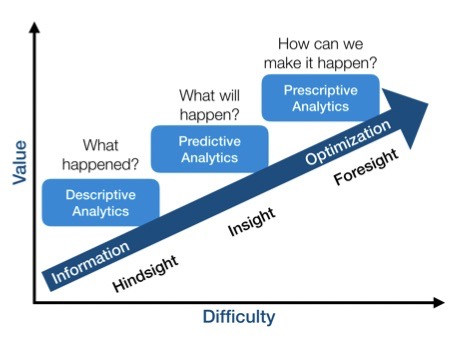
\includegraphics[scale=0.9]{businessAnalytics.jpeg}
\caption{Fasi della business analytics} 
\label{busana}
\end{figure}


% Decisioni
\subsection{Decisioni}

Rappresenta la \hl{scelta di un elemento tra piu' soluzioni} dopo aver ponderato le opzioni.

Possiamo avere più casi d'uso:
\begin{itemize}
	\item \hl{simplest case}: abbiamo \textbf{poche alternative} quindi una semplice scelta
	\item \hl{multple criteria}: abbiamo \textbf{più metri di paragone} delle performance, quindi si dovranno tenere in conto:
	
	\begin{itemize}
		\item \textbf{soluzioni migliori} di altre (dette di Pareto)
		\item \textbf{vincoli} dovuti dai clienti o da casi logistici da gestire (es: spedizioni)
		\item ottimizzazioni matematiche
		\item \textbf{conflitti tra i vincoli}
	\end{itemize}
	
	\item \hl{incertezze e rischi}: 
	
	\begin{itemize}
		\item \textbf{decisioni operative}: di \textbf{breve periodo}  \textbf{reversibili} e \textbf{limitate} a "n" persone del team
		
		\item \textbf{decisioni tattiche}: \textbf{coinvolge una parte dell'organizzazione} per un medio periodo
		
		\item \textbf{decisioni strategiche}: di \textbf{lungo periodo}  \textbf{non reversibili} e \textbf{coinvolgono denaro}
		
		\item \textbf{decisioni strutturate}: hanno una \textbf{procedura di risoluzione specifica}
		
		\item \textbf{decisioni non strutturate}: richiedono \textbf{creatività} ed \textbf{esperienza} in un  dato settore
	\end{itemize}
\end{itemize}

\begin{figure}[H]
\centering
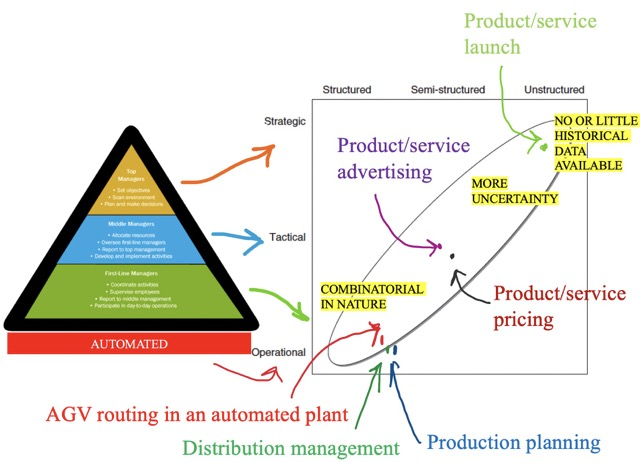
\includegraphics[scale=0.3]{dectax.jpeg}
\caption{Diagonale decisionale} 
\label{diadec}
\end{figure}


% Business Intelligence (BI)
\subsection{Business Intelligence (BI)}

Usato per indicare un \hl{sistema dedicato alla raccolta di dati e alla loro elaborazione} al fine di un reporting, infatti per "Inteligence" si intende investigazione.
Venivano \hl{usati su dati atomici} per avere delle conoscenze approfondite in un determinato business.


% Data visualization
\subsection{Data visualization}

Consiste nel \hl{prendere dati e plottare un grafico}, ma in realtà ora si ha una trattazione più metodologica, cioè se visualizzare in  modo statico o meno i dati.


% Decision Support Systems (DSS)
\subsection{Decision Support Systems (DSS)}

Si indicava un \hl{sistema computerizzato dotato di un sistema di "data managment"} per creare un modello di ottimizzazione, fornendo un feedback tramite un'interfaccia. Ora indica una varietà di sistemi per visualizzare i dati in larga misura o meno.


% Operations Research (OR)
\subsection{Operations Research (OR)}

\hl{Attivita organizzative per portare avanti un sistema logistico}. Per "research" si indica la ricerca delle operation per conseguire dei risultati, avremo come sottocategorie:
\begin{itemize}
	\item \textbf{ottimizzazione matematica}
	\item \textbf{queueing theory}: \textbf{studio matematico delle linee in attesa}  il limite è che funzionano solo con sistemi semplici e con richieste di servizio in ordine stocastico
	\item \textbf{simulazione}: per usarle è \textbf{necessario generare dei numeri randomici}  \textbf{quindi  inconveniente} (bisogna fare un analisi statistica dei risultati dalle quali si farà una \textbf{stima} 
	\item \textbf{game theory}: decisioni con \textbf{più players}
\end{itemize}


% Agents
\subsection{Agents}

È un \hl{sistema che si muove in un environment} (ambiente), ha dei \hl{sensori} tramite i quali percepisce alcuni aspetti del mondo che lo circonda quindi si crea una \hl{rappresentazione del mondo circostante} che può vedere. È capace di \hl{influenzare l'ambiente tramite degli attuatori} come ruote o braccia (intendiamo anche agenti software).

Possiamo classificarli come:
\begin{itemize}
	\item \hl{agenti autonomi}: se è concepito in modo tale che \textbf{tramite un'istruzione sintetica raggiunge un goal sviluppando le azioni per raggiungerlo}  In realtà può anche non essere una sequenza di azioni dato che \textbf{potrebbero esserci degli imprevisti}
	\item \hl{agenti intelligenti}: se
	\item \textbf{impara dall'esperienza}
	\item crea una \textbf{rappresentazione dell'ambiente} che lo circonda e \textbf{ci ragiona sopra} per un possibile risultato delle proprie azioni
	\item \textbf{si adatta ad un ambiente mutevole}
\end{itemize}

\begin{figure}[H]
\centering
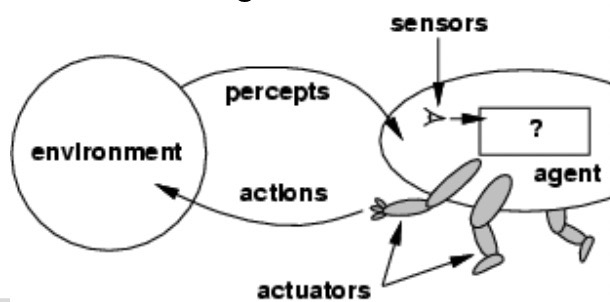
\includegraphics[scale=0.3]{agents.jpeg}
\caption{Schematizzazione di un agente e sue caratteristiche} 
\label{agente}
\end{figure}


% Artificial Intelligence (AI)
\subsection{Artificial Intelligence (AI)}

Comprende tante sottodiscipline:
\begin{itemize}
	\item \hl{automated reasoning}: legato alla \textbf{rappresentazione del mondo} e \textbf{come raggionare su di essa} ma anche calcolandone le probabilità
	\item \hl{automated planning}: usato in ambienti industriali
	\item \hl{automated learning}
	\item \hl{natural language processing}: \textbf{sviluppare agenti software} per fare sintesi di testi, scrivere automaticamente articoli, chat bot, ecc 
	\item \hl{perception}: visione artificiale
	\item \hl{manipuliation}: avere un \textbf{agente che può modificare l'agente} circostante
\end{itemize}


% Machine Learning (ML)
\subsection{Machine Learning (ML)}

Consiste nell'\hl{apprendimento automatico} e quindi lo sviluppo degli \hl{agenti che apprendo tramite la loro esperienza pregressa}. Ci sarà allora una fase di \hl{training}.
Una delle possibili \hl{architetture che permette di farlo sono le Neural Networks} prima avevano solo 2/3 neuroni, ora ne hanno vari strati il che fornisce delle prestazioni impressionanti


% Deep Leaning
\subsection{Deep Leaning}

Si basa sull'\hl{apprendimento automatico} con reti neurale tramite un gran numero di strati di neuroni.


% Data Mining (DM)
\subsection{Data Mining (DM)}

Usare metodi di Machine Learning per \hl{estrarre manualmente dei pattern dai dati}, cioè una \hl{regolarita' o un trend}. È quindi la parte nobile del knowledge discovery in db, dato che i dati sono in genere disponibili su db o da altre piattaforme.

La \hl{sequenza} nella quale interviene è:
\begin{enumerate}
	\item \textbf{prendere} i dati
	\item trovare i vari \textbf{target}
	\item \textbf{preprocessare} i dati
	\item trasformare i dati tramite il \textbf{data mining}
	\item trovare dei \textbf{patterns} (dopo il data mining)
\end{enumerate}

































